\documentclass{article}
\usepackage{import}
\import{../../lib/latex/}{wgmlgz}


\begin{document}

\itmo[
      variant=666666666,
      labn=2,
      discipline=Основы профессиональной деятельности,
      group=P3115,
      student=Владимир Мацюк,
      teacher=Пашнин Александр Денисович
]
\lstset{language=Python}

\tableofcontents

\section{Задание}
По выданному преподавателем варианту определить функцию, вычисляемую программой, область представления и область допустимых значений исходных данных и результата, выполнить трассировку программы, предложить вариант с меньшим числом команд. При выполнении работы представлять результат и все операнды арифметических операций знаковыми числами, а логических операций набором из шестнадцати логических значений.
\begin{center}
      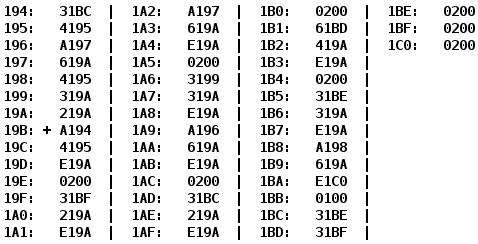
\includegraphics[scale=0.5]{task.png}
\end{center}

\begin{tabular}{|c|c|c|c|} \hline
      Адрес        & Код команды    & Мнемоника & Комментарии \nl
      \texttt{194} & \texttt{31BC}  &  \texttt{}         & \nl
      \texttt{195} & \texttt{4195}  & \texttt{} & \nl
      \texttt{196} & \texttt{A197}  & \texttt{} & \nl
      \texttt{197} & \texttt{619A}  & \texttt{} & \nl
      \texttt{198} & \texttt{4195}  & \texttt{} & \nl
      \texttt{199} & \texttt{319A}  & \texttt{} & \nl
      \texttt{19A} & \texttt{219A}  & \texttt{} & \nl
      \texttt{19B} &+ \texttt{A194} & \texttt{} & \nl
      \texttt{19C} & \texttt{4195}  & \texttt{} & \nl
      \texttt{19D} & \texttt{E19A}  & \texttt{} & \nl
      \texttt{19E} & \texttt{0200}  & \texttt{} & \nl
      \texttt{19F} & \texttt{31BF}  & \texttt{} & \nl
      \texttt{1A0} & \texttt{219A}  & \texttt{} & \nl
      \texttt{1A1} & \texttt{E19A}  & \texttt{} & \nl
      \texttt{1A2} & \texttt{A197}  & \texttt{} & \nl
      \texttt{1A3} & \texttt{619A}  & \texttt{} & \nl
      \texttt{1A4} & \texttt{E19A}  & \texttt{} & \nl
      \texttt{1A5} & \texttt{0200}  & \texttt{} & \nl
      \texttt{1A6} & \texttt{3199}  & \texttt{} & \nl
      \texttt{1A7} & \texttt{319A}  & \texttt{} & \nl
      \texttt{1A8} & \texttt{E19A}  & \texttt{} & \nl
      \texttt{1A9} & \texttt{A196}  & \texttt{} & \nl
      \texttt{1AA} & \texttt{619A}  & \texttt{} & \nl
      \texttt{1AB} & \texttt{E19A}  & \texttt{} & \nl
      \texttt{1AC} & \texttt{0200}  & \texttt{} & \nl
      \texttt{1AD} & \texttt{31BC}  & \texttt{} & \nl
      \texttt{1AE} & \texttt{219A}  & \texttt{} & \nl
      \texttt{1AF} & \texttt{E19A}  & \texttt{} & \nl
      \texttt{1B0} & \texttt{0200}  & \texttt{} & \nl
      \texttt{1B1} & \texttt{61BD}  & \texttt{} & \nl
      \texttt{1B2} & \texttt{419A}  & \texttt{} & \nl
      \texttt{1B3} & \texttt{E19A}  & \texttt{} & \nl
      \texttt{1B4} & \texttt{0200}  & \texttt{} & \nl
      \texttt{1B5} & \texttt{31BE}  & \texttt{} & \nl
      \texttt{1B6} & \texttt{319A}  & \texttt{} & \nl
      \texttt{1B7} & \texttt{E19A}  & \texttt{} & \nl
      \texttt{1B8} & \texttt{A198}  & \texttt{} & \nl
      \texttt{1B9} & \texttt{619A}  & \texttt{} & \nl
      \texttt{1BA} & \texttt{E1C0}  & \texttt{} & \nl
      \texttt{1BB} & \texttt{0100}  & \texttt{} & \nl
      \texttt{1BC} & \texttt{31BE}  & \texttt{} & \nl
      \texttt{1BD} & \texttt{31BF}  & \texttt{} & \nl
      \texttt{1BE} & \texttt{0200}  & \texttt{} & \nl
      \texttt{1BF} & \texttt{0200}  & \texttt{} & \nl
      \texttt{1C0} & \texttt{0200}  & \texttt{} & \nl
\end{tabular}
\section{Вывод}
Я познакомился с форматами файлов JSON, XML и написал парсер JSON на Python .
\end{document}
